\chapter{State of the art}\label{cha:state}
%% Proposed roadmap
%
%   The use of RT in the industrial environments
%   Current standards IEEE and IEC and the TSN
%           Roadmap of standards
%           RTE protocols and OPC UA   
%           How are they related
%  
%   -----------State of the art--------------------------------
%   Applications with RTE and OPC UA in Hard Real Time applications     
%   A brief overview about the RT tools in robotics
%           The importance of EtherCAT as an open RTE protocol within robotics
%   Comparison of openess
%   EtherCAT introduction (selected by Hans Robot)
%           Focus on EtherCAT XoE <<THIS ONLY NEEDS TO BE MENTIONED
%------------------Out of scope--------------------------------------
%   HW ASICS and stuff like that
%   SW Stacks for EtherCAT development and other RTEs
%

This chapter introduces some current applications mainly foucsed on robotics, since this area is closely
related to the environment with which the ACB will be interacting. Robotics sees various advantages
from the RT capable communication protocols, when it comes to integrate motion controllers and 
any other industrial peripheral. Afterwards, an overview about industrial development framworks is 
given, yet focused not on the RT interfaces, but the specific software. The latter is of great importance,
for the Real Time Operative Systems (RTOS) are a corner stone for embedded systems that need to provide a 
deterministic service within their environment. Finally, an overview of the EtherCAT protocol is included.


\section{Current applications}\label{sec:applications}

As rapidly mentioned in \ref{sec:standards}, the SERCOS motion control interface has been standardized within the 
CPFs of IEC 61784-Part 2. Furthermore, it has been even integrated to EtherCAT as a compatible CP. 
This service is available within the DLL and AL and is called Sercos over EtherCAT (SoE), which provides access to motion controllers under 
the SERCOS specifications and, consequently, offers interoperability within its own RT features and the latter's hard RT capabilities.  
An example of this compatibility is presented in \cite{ecat_sercos}, %Motion Control System using SERCOS over EtherCAT
it shows that a jitter of 30 microseconds is feasible in a control loop while the Master uses the SoE service.

Another interesting application has been the characterization of an EtherCAT Master within a Real Time control 
loop for Servo Motors, which run CAN devices over EtherCAT (CoE service). The implementation of the Master device ran on different open source RT OS based on Linux, 
namely, Xenomai and Linux with the \emph{RT\_PREEMPT}. It was concluded that both of the apporaches 
were capable to achieve update periods of $1 ms$ 
, and Jitter around $1.15$ 
microseconds. Moreover, Xenomai could average execution times around 100 microseconds\cite{ecat_xenomai}.%Real-time Servo Control using EtherCAT Master on Real-time Embedded Linux Extensions. 
It is worth to mention that the Master device executed on top of both kernels, the IgH EtherCAT Master, the 
latter mentioned in \ref{sec:openness}.

%85/100
The characterization and optimization of performance of different RTE profiles within TSN is the current topic as the TSN standards and the RTE commisions are still working together,
as briefly mentioned in \ref{sec:standards}. In \cite{tsn_and_sdn} %Integrated Industrial Ethernet Networks: Time-sensitive Networking over SDN Infrastructure for mixed Applications
are presented simulations of TSN topologies with EtherCAT and SERCOS data frames, where the QoS is addressed and evaluated through the usage of SDN (Software-defined Network) for
TSN switches. The approach of this project is to test different scheduling features given fixed Cycle Times of the Data frames, which were proposed to be similar to the current applications
in both technologies. In this manner the importance of an unifed network that supports diferent protocols is highlighted, but further research in this topic, including tests with
other RTE Data Frames is still open.

Besides robotics, a recent industrial application concerning distributed control and monitoring based
on EtherCAT open protocol can be seen in this article \cite{ecat_industrial}.

%90/100
Addressing now the usage of open source tools, OS and RTE Protocols, for development of complex robotic systems, in \cite{ecat_motionplanning} %Motion Planning for Quadrupedal Locomotion: Coupled Planning, Terrain Mapping and Whole-Body Control
is presented a \emph{Motion Planning for Quadrupedal Locomotion}. This is roughly composed, besides the hydraulical actuators, mechanics and other peripherals, of two PCs on board with RT capabilities and shared memory. 
RT Linux (Xenomai) runs on both of them and take care of different levels of the control threads at two different rates depending on the tasks, namely 1 kHz and 250 Hz. The former rate is used
for communicating with the motor controllers over EtherCAT interfaces.

Currently \emph{Han's Robot Germany GmbH} focuses on enhancing robots’ cognitive abilities by developing in the fields of environment perception, drive technologies, 
control theory, material science, mechanical design and artificial intelligence. Interfaces within the robotic system rely on various
industrial protocols to make its interoperability one of the key features. For instance, current motor drivers
are linked over internal EtherCAT chain to the main controller\cite{hans_homepage}.

The above mentioned applications are just a tiny number of examples that shows the importance of an already standardized open industrial communication protocol, 
within a broad set of fields that cannot be completely covered in the scope of this document. Nevertheless, it paves the road to understand why generating the know-how 
to any of the mentioned technologies, represents a high-impact resource for any research or development group, regardless of its commercial or academic purposes.

\section{An overview about the RT capable SW in robotics}

As the previous section was being written, several resources and examples showed the current usage of RT-oriented
open source software an its community. Since this Research Project has a goal of introducing the reader a roadmap for RTE communication interfaces and 
its applications, it was worth adding this section to summarize the RT Software for development in robotics.

As mentioned in \cite{ecat_xenomai} and \cite{ecat_motionplanning},%the robot examples
the usage of middlewares within the field of robotics is growing and it relies on robot software that exists between the application and a RT capable OS.
In \cite{middleware_industrial} %2020-Real-Time Robot Software Platform for Industrial Application
a list of requirements is provided to address these middlewares and how to consider them Real Time Robot Software Platforms. The mentioned list can be interesting
to start getting familiar with the capabilities and features of the so-called Robot Software. The list of requirements is as follows: 
\begin{itemize}
    \item R1: Support data exchange
    \item R2: Real time support (strict period execution and sporadic performance support)
    \item R3: Supports thread and process types for user defined programs
    \item R4: Easy configuration of applications (robot control SW, PLC SW, vision inspection SW, non-real-time SW, etc.)
    \item R5: Support multiple periods.
    \item R6: Threads or processes running in the same period are classified by priority.
    \item R7: Check and handle the event through the event handler.
\end{itemize}

Common names for different projects aiming to create this development frameworks are the following: Common Object Request Broker Architecture
(CORBA), Real-Time CORBA (RT-CORBA), Data Distribution Service (DDS), OPC Unified Architecture (OPC-UA), Robot Operating System
(ROS), Open Platform for Robotic Services (OPRoS) OpenRTM (open robotics technology middleware), open robot control software (OROCOS), 
XbotCore, and real-time middleware for industrial automation devices (RTMIA). Further comments and comparison between their features
can be seen in the previously referenced paper. As to what concerns to this document, only some of them will be roughly commented
as they ended up being somehow related to the RTE profiles\cite{middleware_xbotcore}.

\begin{description}
    \item[OPC UA] As frequently mentioned before, this is an open standard for data sharing among nodes within industrial networks and has
    been considered in some projects related to robotics. Neverthless, it is important to highlight that this is no considered a full 
    middleware, since it only provides a protocol to control the exchange of data between nodes, a good degree of reliability and security.
    However, it does not provide RT capabilities to the system only compatibility. Hence, it needs an operative system and the consequent 
    lower layers capable of RT scheduling and communication, concerning the latter the TSN set for protocols is an example.
    \item[ROS/OROCOS/OpenRTM] These are projects that aim to create a suitable middleware for robots by implementing Xenomai or Linux operating systems. 
    ROS prioritizes the final user, avoiding in the way some fine-grained features due to its difficuty, therefore having sometimes
    issues to meet the hardt RT requirements. Orocos has further improved its comaptibility, similarly to OpenRTM.
    \item[CODESYS and TwinCAT] To fully meet compatibility with the industry, the so-called PLC Software has been also used in open robotics.
    These applications roughly need to run both, the robot functional blocks and the robot tasks. For further details on it the following
    references can be reviewed \cite{middleware_xbotcore} and \cite{middleware_xbotcloud}. %referemces from the italian robot Xrobotcore
    \item[xbotcore] This is an attempt to provide of a highly compatible open middleware for industrial robotics, it runs over the Xenomai and 
    uses a SOEM stack to interface with any compatible industrial device, recall \ref{sec:openness}. % XBotCore: A Real-Time Cross-Robot Software Platform 
    Applications has been already mentioned in \ref{sec:applications}, which have reached control loops down to 1khz for 33 axes \cite{middleware_xbotcore}.
    \item[RTMIA] RTMIA middleware + Linux or Xenomai but used open PLC running parallely[?] << This needs further reading [?]
\end{description}


The previous information was presented only to draw an idea for the non-familiar reader about the applications and, since this topic is in on going development 
and, furthermore, many other plataforms are addressing similar challanges are arising; the reader is invited
to go deeper into these topics, for instance, by reviewing this resource \cite{middleware_industrial}. %add the resouce fromt he open community 

\section{Approaching openness within the RT protocols}\label{sec:openness}

Among the industrial standards mentioned in \ref{sec:standards}, there are some related initiatives to include a certain degree of open source
software to improve the development of applications. The following is a brief list of a few interesting references to them. 
However, as expected, most of the software stacks
for industrial communication systems are commercial and provided by third-party companies. 

%90/100
\begin{description}
    \item[OSADL] Open Source Automation Development Lab eG (OSADL):It is a German group that intends to lead the development of open source development
    for industrial automation. Closely related in the developing of OPC UA and other Linux features for industrial applications.
    \item[open62541] Within the official scope of OPC UA, there is this Certified SDK project that is within its second phase, at which it is expected 
    from the research and industrial community to develop applications to test its performance. Moreover, as the TSN specification is of huge importance, 
    a set of enhancements for the \emph{open62541} project were developed by \emph{Fraunhofer IOSB} and a serie of patches for the Linux kernel has been released to 
    make it a RT compatible.\cite{open62541_homepage} %https://www.osadl.org/OPC-UA-over-TSN.opcua-tsn.0.html 
    The OPC UA is developed under GPL 2.0 license and due to its current phase implies a further adaptation for the physical node, e.g., ARM arquitechtures 
    to make them compatible with the mentioned patches. 
    \item[SOEM/SOES] RT Labs Industrial development group focused on Software Stacks for industrial protocols. Among their commercial communication stacks
    there are software stacks under GPL for EtherCAT Master and Slave devices SOEM/SOES*. \cite{soesm_homepage} %https://rt-labs.com/product/soes-ethercat-slave-stack/ 
    \item[Sercos Stacks] Sercos III technology is able to be operated in a common TSN-based network \cite{sercos_tsn}, % Ethernet TSN heralds a new era of industrial communication
    since its development group is working closing together with the TSN group. 
    They also made available open source software dedicated for development of master and slave devices, namely: Common Sercos Master API (CoSeMa),
    Sercos Internet Protocol Services (IPSS), and The Sercos III SoftMaster, the later even allows the host to use any standard Ethernet controller.\cite{sercos_stacks} %https://www.sercos.org/technology/implementation/driver-software/. 
    It is important to mention that there are testing tools to certificate those devices and achive a Safety Integrity Level 3 (SIL-3).
    \item[EtherNet/IP Stacks] There are several commercial stacks that comply with the Open DeviceNet Vendors Association's (ODVA) EtherNet/IP specification. 
    \emph{OpEner} is an open source alternative which targets PCs with a POSIX operating system and a network interface. 
    Examples are provided for integration only in Linux and Windows in \cite{opener_stack}; %http://eipstackgroup.github.io/OpENer/index.html
    nevertheless, a variation for embedded systems has been presented for an STM32 microcontroller. In the mentioned project, more tools had to be adapted, for instance,
    STM32F4x7 Ethernet Driver v1.1.0, lwIP v1.4.1 (TCP/IP Stack), MicroHTTP v5.1.0.1, a patched version of OpENer v1.2., among others.\cite{opener_stm32}%https://www.emb4fun.de/archive/chibiosopener/index.html
    \item[IgH EtherCAT Master] This is a bundle of libraries to give a Linux host (LinuxCNC for example) EtherCAT Master features, it is developed under the GPLv2 license. 
    An interesting example of this open source resource within an Airbus Test Rig can be reviewed in the following reference \cite{ecatstack_igh}. %https://etherlab.org/en/success/airbus-testrig.php
\end{description}

As the scope of this Research Project is only focused on the indsutrial communication profiles capable of RT and, so far has been clear how 
the EtherCAT is a reliable one, yet open and significantly considered in the industry -recall -\ref{sec:applications}-; it makes sense to present an introduction to the protocol itself. 
This way it is easier to go sensibly to the implementation of what is one of the basic chain-elemnts in what could become a very complex application: 
an EtherCAT Slave device with open source elements.

\subsection{EherCAT protocol}\label{sec:ecat_protocol}

As mentioned in the introduction, EtherCAT is an industrial Communication Profile developed by Beckhoff that is 
standardized in the IEC 61588 under the RTE CPF. The development within this company is oriented to the use of 
open standards to increase its impact within the indsutry, but not only reduced to it but the overall field of smart cities[?], in
a certain degree this apporach eliminates the need for many expensive "black boxes"\cite{beckhoff_automation}. %%Beckhoff_Urban_Automation_2013_e almost the introduction thing 
This implies that the interoperability of devices is almost guaranteed, at least from the specification perspective,
not only for private development centers but also for any other developer that follow the standards; if the standards 
are of public access, then this is a mean of empowerment of any group that might be willing
to create its own industrial-compatible technologies.

The OSADL emphatized in 2008 \cite{beckhoff_vs_osadl}, for example, a vision for leading the integration
of opensource in the industry by using the Linux Kernel as a certified Industrial RT (IRT) operative system for industrial embedded applications. 
Back in that day, Beckhoff was involved in that discussion representing the contrary model. Nonetheless, in the last months the same company has
apparently retaken the opensource iniciative by the introduction of the FreeBSD compatible version of the TwinCAT Runtime\cite{beckhoff_freebsd}.%https://www.heise.de/newsticker/meldung/Open-Source-trifft-die-Industrie-201855.html
%**https://www.beckhoff.com/english.asp?highlights/twincat-bsd/default.htm

In comparison with other RTE profiles, EtherCAT has shown a higher performance, more flexible topology and lower costs than other ethernet fieldbus 
technologies. This  protocol  applies  a  master-slave  mode,  in  which  the  master  
device  uses  standerd  100BASE-TX  ethernet  adapter  and  the  ESC  (EtherCAT  Slave  Controler), that implements a EtherCAT IP 
(intellectual property) core within an ASIC or a FPGAto process the frames. As  the  working  cycle starts, the  EtherCAT master  
publishes a frame encapsulated a standardized 8802.3 frame. When the it reaches an ESC, it analyses the address and location on the frame, decides
which parts of it are useful sections and then reads or writes data on it. As the
read-write operation finishes, the Working Counter (WKC) at the end of the frame is added by one, this way the data on the frame has been processed. 
This cycle repeats for each ESC within the topology.%Motion Control System using SERCOS over EtherCAT
EtherCAT supports almost all kinds of topology structure, such as ring, line, star and tree. The transmission speed of  EtherCAT  is  fixed  to  100  
Mbit/s  with  full  duplex  communication.  The  EtherCAT  network  is  able  to  connect  maximally 65535  devices  via  switch  and  media  converter.  
The  EtherCAT  system  can  update  1000  I/Os  in  just  30  microseconds  or  exchange  1486  byte  contents  in  300  microsecond. \cite{beckhoff_datasheet}\cite{ecat_sercos}  %Motion Control System using SERCOS over EtherCAT

Important to highlight is that other CPs are also integrated as services inside the protocol, as previously mentioned for 
the SERCOS specification in \ref{sec:applications}. 
Other examples of these integrated CPs are File over EtherCAT (FoE) or Ethernet over EtherCAT (EoE), which
make possible to support a wide variety of devices and application layers in the same network\cite{beckhoff_compatibility}. %https://www.ethercat.org/en/technology.html#1.9
A complete list of the communication profiles that are on hand
through the protocol's mailboxing is given below, as to the overall layered integration can be seen in figure \ref{fig:ecatprofiles}.
\begin{itemize}
    \item CoE: CAN application protocol over EtherCAT
    \item SoE: Servo drive profile, according to IEC 61800-7-204 (SERCOS protocol)
    \item EoE: Ethernet over EtherCAT
    \item FoE: File Access over EtherCAT (HTTP,FTP,etc)
    \item AoE: Automation Device Protocol over EtherCAT (ADS over EtherCAT)
\end{itemize}

\begin{figure}[ht]
    \centering
    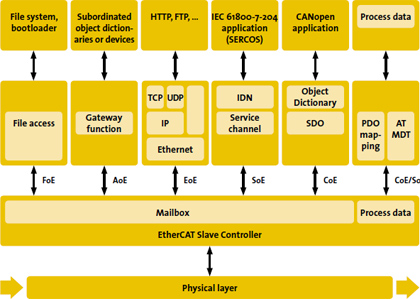
\includegraphics[width=.65\textwidth]{imgs/intro-ecatprofiles.jpg}
    \caption{Different communication profiles can coexist in the same system.}
    \label{fig:ecatprofiles}
\end{figure}

An EtherCAT device with switchport properties usinge EoE would be the equivalent of the TSN compliant
switches, since they would insert any non time-senstitive TCP/IP fragment into the EtherCAT traffic preventing
in this way the real time properties from being affected. Furthermore, the architecture of the protocol itself and
its early cooperation with the IEEE 802.1 group and the OPC Group ensure its continuos compatibility with the
standardization of TSN, OPC UA and the IoT paradigm.\cite{beckhoff_compatibility}%https://www.ethercat.org/en/technology.html#1.12

A slave device must comply at least with CoE and the Mailbox, whereas the Master may comply with all the communication profiles. This of course
needs to be suited to the requirements of the application and the degree of tlexibility that is to be achieved. Consequent certification process
should adhere to Beckhoff's specifications.\cite{beckhoff_slavetutorial} %<< Add the reference to the implementation guide of beckhoff

Having presented this brief summary of the EtherCAT technology, the reader may continue to the following chapters. 
More detailed information of the protocol itself that was needed to understand the function of the SOES library
can be read in the section \ref{sec:soes}.


% *Add the image of the Ethernet frame having the EtherCAT datagram inside.
% *Explain the XAE tool and the PDI meaning
% *Quote maybe from paper section BASICS OF ETHERCAT AND PROFINET IRT Network Delay Analysis of EtherCAT and PROFINET IRT Protocols***



